\documentclass[10pt,conference,compsocconf]{IEEEtran}

\usepackage{hyperref}
\usepackage{fullpage}
\usepackage{times}
\usepackage{fancyhdr,graphicx,amsmath,amssymb}
\usepackage[ruled,vlined]{algorithm2e}
\usepackage{mathtools}
\usepackage{graphicx}	% For figure environment
\usepackage[english]{babel}
\usepackage{comment}

\newtheorem{theorem}{Theorem}
\newtheorem{lemma}[theorem]{Lemma}

\begin{document}
\title{Difference between SGD and random reshuffling}

\author{
  Monde, Diego; Voracek, Vojtech and Wohlleben, Kilian\\
  \textit{Faculty of Computer Science, University of Vienna, Vienna}
}

\maketitle

\begin{abstract}
In this document we will present the difference between stochastic gradient descent and random reshuffling and conduct some experiments to test their performance in different settings.
\end{abstract}

\section{Motivation}
\label{sec:motivation}
\medskip

We first consider unconstrained, finite-sum minimization problems or an
empirical risk minimization; something that is very common in practice:

\begin{equation}\label{eq:finite-sum}
\min_{x \in \mathbb{R}} f(x) = \sum_{i = 1}^n f_i(x),
\end{equation}


\noindent where $f$ is a strongly convex function which ensures that there
exists a unique optimal solution which is denoted by $x^*$. We also assume
that each individual function $f_i$ is smooth with Lipschitz gradients and
\mbox{$L$-Lipschitz} on a bounded domain. This assumption helps us to make
a particular convergence analysis.
These types of problems are common in many areas of machine learning, one example being Linear Regression.

\medskip

Gradient descent~\cite{GD}:
Traditional approach to minimizing convex functions.

\begin{algorithm}
\SetAlgoLined

  $x:= x_0$ \\
 \For{epochs \texttt{t=1,...,T}}{
    $x_{t+1} := x_t - \alpha \nabla f(x_t)$
 }
 
 \caption{Gradient descent}
\end{algorithm}
\noindent A initial vector $x_0$, a number of epochs $T$, and
a step size $\alpha$ are defined by the user.

\medskip

Drawback of gradient descent: For large $n$ it is computationally
expensive to evaluate the full gradient.

Instead of GD one can use the Stochastic gradient descent~\cite{SGD} since
$\nabla f(x) = \sum_{i=1}^n \nabla f_i(x)$.

\begin{algorithm}
\SetAlgoLined

  $x:= x_0$ \\
 \For{epochs \texttt{t=1, ..., T}}{
    \For{\texttt{i=1, ..., n}}{
      Sample $j \in \{1,..., n\}$ uniformly.
      $x_t^{i+1} := x_t^i - \alpha \nabla f_j(x_t^i)$
    }
    $x_{t+1} = x_t^n$
 }
 
 \caption{Stochastic gradient descent}
\end{algorithm}

\medskip

Drawbacks of SGD and also the motivation to introduce Random
reshuffling~\cite{COMPONENTFUNCTION}:

\noindent The specific sample may be chosen more frequently than others. On the
other hand, Random reshuffling guarantees that all samples are selected at
the same frequency.

\medskip

\noindent Random reshuffling:

\noindent In each epoch $t$, we sample indices $[\pi_1, \pi_2,..., \pi_n]$
without replacement from $\{1, 2,..., n\}$, in other words,
$[\pi_1, \pi_2,...\pi_n]$ is a random permutation of the
set $\{1, 2,..., n\}$ and than perform $n$ iterations of the following
form

$$x_t^{i+1} := x_t^i - \alpha \nabla f_{\pi_i}(x_t^i)$$

\begin{algorithm}
\SetAlgoLined

  $x:= x_0$ \\
 \For{epochs \texttt{t=1, ..., T}}{
    Sample a permutation \\ $[\pi_1, \pi_2,...,\pi_n]$
    of $\{1, 2,...,n\}$ \\
    \For{\texttt{i=1, ..., n}}{
      $x_t^{i+1} := x_t^i - \alpha \nabla f_{\pi_i}(x_t^i)$
    }
    $x_{t+1} = x_t^{n+1}$
 }
 
 \caption{Random reshuffling}
\end{algorithm}

\section{Optimization problems}

We start with some benchmark functions to analyze the difference between
SGD and RR. Then we use those algorithms to solve two real-life problems.

\subsection{Sphere function}

\noindent Definition~\cite{SPHERE}:
$$f(x) = \sum_{i=1}^n x^2$$
Components of gradient:
$$\nabla f_i(x) = [0,...,0,2\cdot x_i,0,...,0]$$
Global minimum:
$$f(x^*) = 0$$
$$x^* = [0,...,0]$$
Strong-convexity constant $\mu = 2$, Lipschitz constant \mbox{$L=2$},
number of components of the gradient: $n$. It is presumable one of
the easiest continuous domain optimization problem.

\subsection{The component function}
\noindent Definition~\cite{COMPONENTFUNCTION}:
$$f_1(x) = \frac{1}{2}(x-1)^2, f_2(x) = \frac{1}{2}(x+1)^2 + \frac{x^2}{2}$$
$$f(x) = f_1(x) + f_2(x) = \frac{3}{2} x^2 + 1$$
Components of gradient:
$$\nabla f_1(x) = x - 1, \nabla f_1(x) = 2x + 1$$
Global minimum:
$$f(x^*) = 1$$
$$x^* = 0$$
Strong-convexity constant $\mu = 3$, Lipschitz constant \mbox{$L=3$},
number of components of the gradient: 2. This is an example of a function where RR is provably better than SGD. \cite{COMPONENTFUNCTION}

\subsection{Least squares linear regression}

\noindent Definition~\cite{REGRESSION}:
$$f(x) = \sum_{i=1}^n (A^T x_i-b)^2 = ||A^T x-b||^2,$$
\noindent where $A \in \mathbb{R}^{n \times d}$ and $b \in \mathbb{R}^{n
\times 1}$ are to be learned.
Components of gradient:
$$\nabla f_i(x) = 2 A(A^T x_i - b)$$
Global minimum:
$$f(x^*) = ||A (A^T A)^{-1} A^T b - b||$$
$$x^* = (A^T A)^{-1} A^T b$$
Strong-convexity constant $\mu = \lambda_{min}(2A^TA)$, Lipschitz constant
\mbox{$L=\lambda_{max}(2A^TA)$}, where $\lambda_{min}(\cdot),
\lambda_{max}(\cdot)$ denotes the smallest and the largest
eigenvalues. respectively. The number of components of the gradient: $n$.

\subsection{Neural Network}
\noindent Definition~\cite{NEURALNETWORK}:
$$f(x) =  A_{n} \sigma_n(A_{n-1}\sigma_{n-1}(... A_0 x + b_0)) + b_{n-1}) + b_n,$$
\noindent where $\sigma_i$ is a non affine function. 

Here we have a non convex function without a clear optimal solution. The gradient is obtained via the chain rule and the number of components is equal to the number of samples. 


\section{Experiments}


\medskip

In this work, we use the step size $\alpha = c / (t+1)^s$, where $c>0, s \in (0, 1]$ for the t-th epoch. If we consider q-suffix\footnote{q-suffix
average is obtained by averaging the last $qk$ iterates at iteration
$k$~\cite{COMPONENTFUNCTION}} averages of the iterates for some $q \in (0,1]$
and step size $\alpha = c / (t+1)^s$, one can show in the convex case that those iterates of both algorithms (SGD, RR) converge almost surely  at rate
$\mathcal{O}(1 / t^s)$ to the optimal solution~\cite{COMPONENTFUNCTION}.
The specific requirements on the functions $f_i$ described in
the~\ref{sec:motivation}~section are necessary to prove this.


The aim of this work is to compare performance of RR and SGD on
specific functions~\ref{eq:finite-sum}. For this purpose, we measured the
performance of those two algorithms on the Sphere function of different
dimensions, on the component function and on the real-world
Linear and Neural Network Regression - the Diabetes dataset provided by
sklearn~\cite{DIABETES,SKLEARN}. For the diabetes dataset, the dimension
is 10, and the optimized function is a sum of 442 independent functions.

\section{Results}
Here we see plots of the training for the different problems. Our main interest are the bold red and blue lines that show the average of all the runs. The graph shows the distance of q-suffix average $\overline{x}_{q,k}$ to the optimal solution $x^*$ during training. Moreover, the curve capturing the convergence rate $\mathcal{O}(1 / k^s)$ is added. Where we don't know the optimum, i.e. in the neural network case, we look at the objective function. 

\begin{figure}[h]
  \centering
  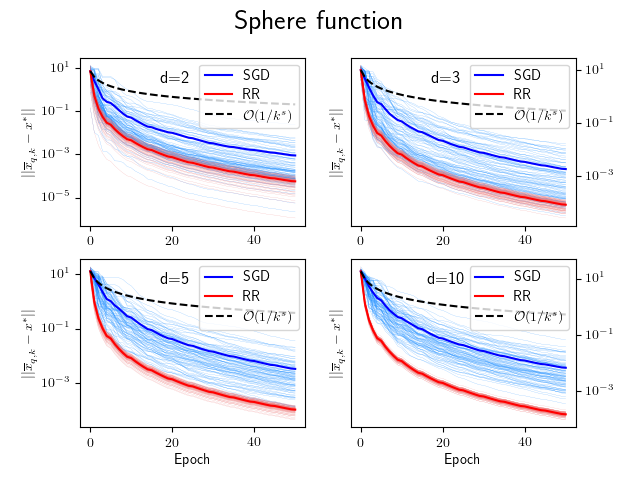
\includegraphics[width=\columnwidth]{Sphere_function_runs}
  \caption{Here we see, that RR outperforms SGD quite clearly. The results of RR vary little and stay equal for different dimensions, while SGD gets visibly worse as d gets larger. }
  \vspace{-3mm}
  \label{fig:squareav1}
\end{figure}

\begin{figure}[h]
  \centering
  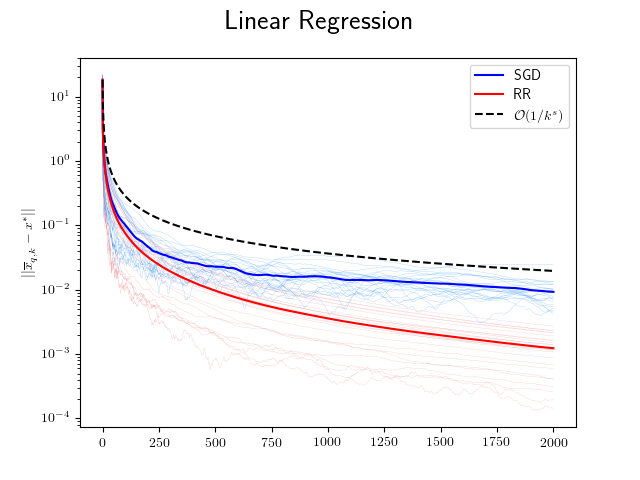
\includegraphics[width=\columnwidth]{Linear_Regression_run}
  \caption{Here we see, that on average RR leads to better results than SGD. In particular we see that SGD barely improves after a certain point, while RR is still improves after 2000 epochs.}
  \vspace{-3mm}
  \label{fig:leastsquares1}
\end{figure}

\begin{figure}[h]
  \centering
  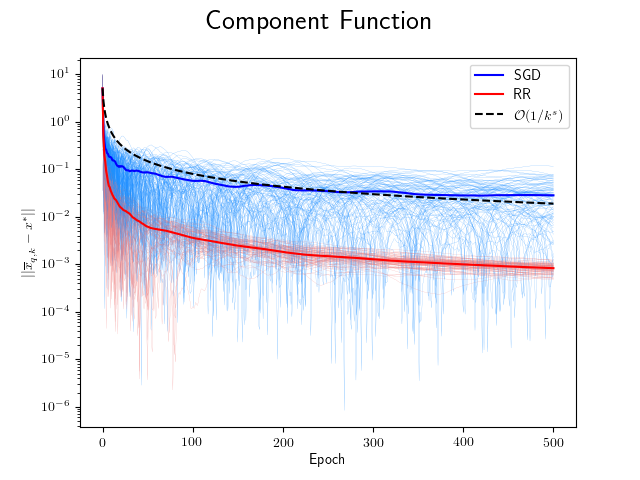
\includegraphics[width=\columnwidth]{Component_Function_run}
  \caption{For the component function we see that indeed RR outperforms SGD very quickly and quite significantly with over an order of magnitude. Again we see less variance between the different trainings.}
  \vspace{-3mm}
  \label{fig:component1}
\end{figure}

\begin{figure}[h]
	\centering
	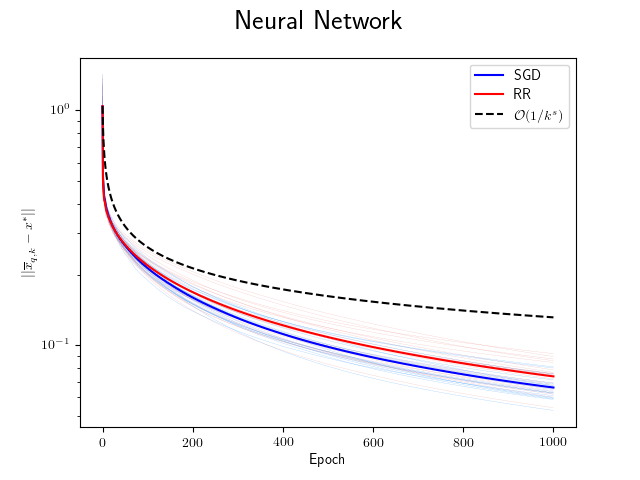
\includegraphics[width=\columnwidth]{Neural_Network_run}
	\caption{In the neural network case we actually have that SGD performs better. While it is barely visible in this picture, the data shows, that initially RR improves quicker but at some point SGD takes over. }
	\vspace{-3mm}
	\label{fig:nonconvex1}
\end{figure}

\section{Conclusion}

RR has outperformed SGD in all our convex experiments. We have specifically seen, that RR is much more stable and yields faster convergence. In the case of the sphere function that is due to the fact that all components of $x$ are optimized over equally often, so that no dimension is "neglected". In the case of the component function we could confirm the theoretical superiority of RR proven in \cite{COMPONENTFUNCTION}. For the real world dataset, we have also seen, that optimizing over the entire dataset uniformly is better than leaving the frequency to chance in the convex case, however in the non-convex case, SGD outperformed RR. That is likely due to SGD being better able to escape saddle points in this case, however that is only a conjecture and not confirmed. Initially RR decreases faster but is surpassed by SGD at a later point. 

\section{Appendix}

\noindent Settings for the experiments.

\medskip

\noindent Sphere function:

\begin{itemize}
	\item $\text{max epochs} = 50$
	\item $q = 0.2$
	\item $ \text{runs} = 100$
	\item $s = 0.9$
	\item $c = 1$
	\item $x_0 \sim {\cal U}_{[-10, 10]}^d$
\end{itemize}

\medskip

\noindent Component function:

\begin{itemize}
	\item $ \text{max epochs} = 500$
	\item $q = 0.2$
	\item $ \text{runs} = 100$
	\item $s = 0.9$
	\item $c = 1$
	\item $x_0 \sim {\cal U}_{[-10, 10]}$
\end{itemize}

\medskip

\noindent Linear regression:

\begin{itemize}
	\item $\text{max epochs} = 2000$
	\item $q = 0.2$
	\item $\text{runs} = 25$
	\item $s = 0.9$
	\item $c = 0.1$
	\item $x_0 \sim {\cal U}_{[-10, 10]}^{442\times10}$
\end{itemize}

\medskip

\noindent Neural Network:

\begin{itemize}
	\item $\text{max epochs} = 2000$
	\item $q = 0.2$
	\item $\text{runs} = 20$
	\item $s = 0.3$
	\item $c = 0.03$
	\item $\text{no hidden layers} = 2$
	\item $\text{no neurons} = (50,40)$
	\item $A_i \sim {\cal N} (0, \frac{2}{\text{dim in} + \text{dim out}})$
	\item $b_i = 0$
	\item $\sigma_i = \text{Leaky ReLU with } \alpha = 0.1$
\end{itemize}

\newpage
\bibliographystyle{IEEEtran}
\bibliography{references}

\end{document}
